\documentclass[a4paper]{article}

\usepackage[frenchb]{babel}
\usepackage[T1]{fontenc}
\usepackage[utf8]{inputenc}
\usepackage{amsmath}
\usepackage{graphicx}
\usepackage{lmodern}
\usepackage[left=3cm, right=3cm, bottom=4cm, top=4cm]{geometry}
\usepackage{array}
\usepackage{pdfpages}
\usepackage{listings}
\usepackage{enumitem}
\usepackage{color}
\frenchbsetup{StandardLists=true}
\usepackage{pifont}

\usepackage[gen]{eurosym}
\DeclareUnicodeCharacter{20AC}{\euro{}}

\usepackage{hyperref}
\hypersetup{    
    colorlinks,
    citecolor=black,
    filecolor=black,
    linkcolor=black,
    urlcolor=black
}

\title{Rapport de spécification}

\author
{
	Pierre-Marie {\sc Airiau}\\
    Valentin {\sc Esmieu}\\
    Hoel {\sc Kervadec}\\
    Maud {\sc Leray}\\
    Florent {\sc Mallard}\\
    Corentin {\sc Nicole}
}

\date{\today}

\newcommand{\pagevierge}[0]{\newpage\thispagestyle{empty}\null\newpage}

% Rapport de spécification fonctionnelle
%     Français
%     Décrire en détail les spécifications fonctionnelles du prj
%     Première idée architecture logicielle générale
%     décrire les grands modules et leur intéraction
%     Repart travail existant: Doit faire état tests effectués
%     Environ 20 pages


\begin{document}
    % Ouh c'est sale.
    \hypersetup{pageanchor=false}
    
\includepdf[pages=1]{figure/couv.pdf}
    \hypersetup{pageanchor=true}
    
    \newpage
    \thispagestyle{empty}
    \mbox{}
    
    \newpage
    % A decommenter pour la release
    % \setcounter{tocdepth}{2}
    \tableofcontents
    \setlength{\parskip}{10pt}
    
    \newpage
    \thispagestyle{empty}
    \mbox{}

    \newpage
    \section{Introduction}
	La sécurisation des systèmes est une problématique majeure de la société moderne. En ce sens, de nombreuses méthodologies ont été développées~\cite{introSecurite,ADTreeKordy} dans le but d'identifier les risques et de les quantifier. C'est avec cet objectif que le concept d'arbres d'attaque et de défense (ADTrees) a vu le jour.

	Lors de la phase de pré-étude, nous avons pu comprendre l’intérêt pratique de la construction des ADTrees. Leur utilisation permet d'identifier de manière précise les différentes attaques possibles contre un système et de les valuer en termes de coût, de probabilité, etc. ADTool~\cite{adtool_paper} (Attack-Defense Tree Tool), un logiciel libre développé pour l'implémentation de ces arbres sur support informatique, a été mis à disposition pour ce projet. Lors de sa prise en main, des limites ont été constatées. En effet, dans un cas concret d'expertise en sécurité, le système doit faire face à une multitude d'attaques possibles et, par conséquent, l'ADTree qui les modélisera sera de très grande taille. Dans ce cas, il est très difficile pour l'expert d'en extraire des informations pertinentes au premier coup d’œil. Or, ADTool ne fournit pas d'outil permettant à l'utilisateur de simplifier l'analyse de l'arbre. 

	L'objectif de ce projet est donc la création d'un logiciel intégrant ADTool et permettant de faciliter le travail d'un expert en sécurité, en lui fournissant des outils pour analyser facilement ses ADTrees. Ce logiciel portera le nom de \glasir{}  (prononcé [\textipa{glaziK}]). Il s'agit du nom d'un arbre aux feuilles d'or dans la mythologie nordique~\cite{vikingCulture}.

	Ce rapport présente les spécifications fonctionnelles de \glasir{}. Tout d'abord, les limites d'ADTool seront abordées, afin de justifier l'intérêt de \glasir{}. Puis nous détaillerons les différentes fonctionnalités destinées à l'analyse des ADTrees. Enfin, quelques améliorations supplémentaires seront également précisées pour offrir un meilleur confort de création et édition d'arbres. Ces spécifications seront faites en prenant en exemple une situation précise : celle d'un expert en sécurité chargé par le Service des Transports en commun de l'Agglomération Rennaise (STAR) de déterminer les failles de leurs systèmes de paiement.

    \section{\'Etude de l'existant}
	\label{sec:adtool}

	% Hierarchiser cette partie
	% Mettre en évidence fct qui manquent 

	ADTool permet de construire un ADTree sans difficulté. Le logiciel offre la possibilité de créer de nouveaux nœuds, d'éditer leurs labels et de leur ajouter des fils et des frères de façon simple et intuitive. Le choix des opérateurs entre ces nœuds --- conjonction ou disjonction ---  se fait sans effort, et la mise en place de défenses est également réalisable très facilement. % + figure ?
	
	\begin{figure}[h]
        \centering
        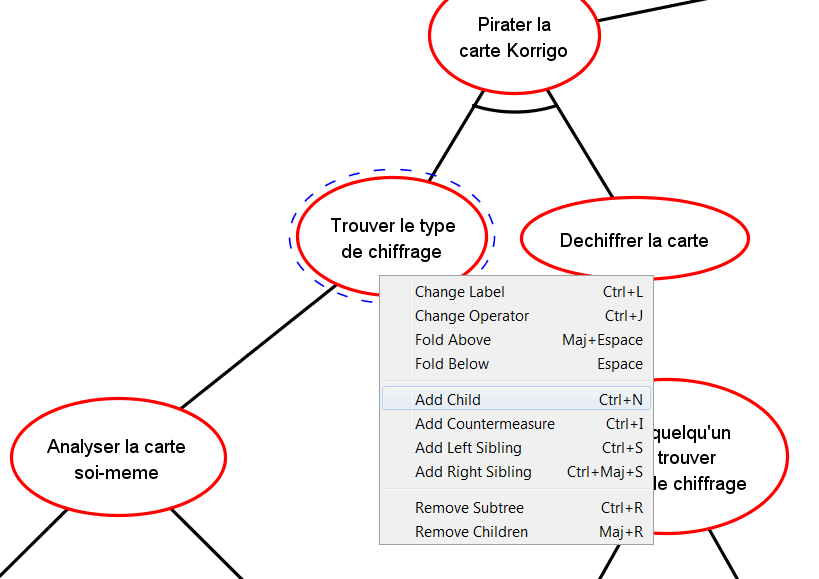
\includegraphics[width=1\textwidth]{figure/adtool_add_child.png}
        \caption{La création d'un arbre dans ADTool est simplifiée par des actions accessibles facilement.}
        \label{fig:arbre_exemple_1}
    \end{figure}
	
	Une fois l'arbre établi, il est possible d'ajouter des valuations à chaque feuille\footnote{Une feuille est un nœud n'ayant aucun fils.} de l'arbre selon un paramètre de base, tel que le coût minimal, la probabilité de succès, etc. (voir Section \ref{sec::ParamBase}). ADTool se charge ensuite de propager les valuations aux nœuds pères de façon récursive, jusqu'à la racine. % ajout de la liste des paramètres ?
	
	\begin{figure}[h]
        \centering
        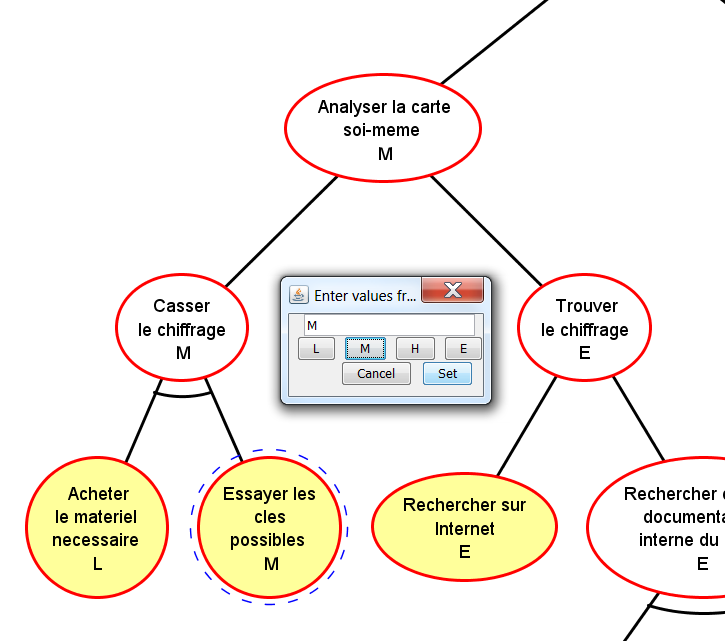
\includegraphics[width=1\textwidth]{figure/adtool_add_values.png}
        \caption{L'ajout de valuations aux feuilles est simple. Ces valuations se propagent ensuite récursivement à tous les antécédents }
        \label{fig:arbre_exemple_1}
    \end{figure}
	
	Dans l'exemple de la {\sc Figure} \ref{fig:arbre_exemple_1}, chaque noeud possède une valuation selon le paramètre de base \og difficulté de réalisation \fg{}. Cette valuation peut prendre la valeur L, M, H ou E ((\emph{Low}, \emph{Medium}, \emph{High} ou \emph{Extrem} --- voir Section \ref{sec::ParamBase} pour plus de détails). En éditant la difficulté de réalisation de la feuille \og essayer les clés de chiffrage possibles \fg{}  à \emph{Medium}, la valuation du nœud père \og casser le chiffrage \fg{} est recalculée pour prendre la valeur \emph{Medium} : en effet, la difficulté de ce nœud conjonctif correspond à la difficulté la plus élevée parmi ses fils. Puis, à son tour, la valuation du père de ce nœud-père est recalculée à \emph{Middle}, car, étant un nœud disjonctif, sa difficulté de réalisation correspond à la difficulté la plus faible de ses fils.
	
	L'utilisateur n'a donc pas de calcul à faire lui-même pour obtenir la valuation de la racine de son arbre, c'est-à-dire la valuation de son objectif final. Cependant, l'analyse de l'arbre ainsi construit ne va pas plus loin : ADTool ne précise pas d'où provient la valuation d'un nœud. % mettre en évidence
	 Par conséquent, l'utilisateur n'a aucun moyen de déterminer le \og meilleur chemin \fg{} permettant d'atteindre la racine de l'arbre, par exemple. Il doit donc le déduire manuellement, en analysant comment les valuations se sont propagées. Sachant qu'un arbre atteint très rapidement une taille conséquente, cette opération peut prendre un temps très important, ce qui peut être un obstacle pour l'utilisateur.
	
	L'analyse de l'arbre est également restreinte par le fait que la valuation d'un nœud ne peut se faire que selon un seul paramètre. Il n'est pas possible de prendre en compte la \og difficulté \fg{} ET le \og temps nécessaire \fg{} à la réalisation d'un nœud, par exemple. Ceci est contraignant car il est difficile de séparer ces deux notions : par exemple, le nœud \og essayer les clés de chiffrage possibles \fg{} est très facile à effectuer (il suffit de taper les clés une-à-une jusqu'à trouver la bonne), mais le temps nécessaire pour effectivement essayer chaque clé est colossal. ADTool ne permet donc pas d'obtenir une vision plus complète de l'arbre par combinaison de plusieurs paramètres. % 2eme limitation : mettre en évidence.
	
	 De plus, lorsque l'utilisateur souhaite se focaliser sur une partie de son arbre, il ne peut que masquer tous les nœuds hiérarchiquement au-dessus (ou en dessous) d'un nœud spécifique, % 3ème limitation : mettre en évidence.
	  sans distinction. Il pourrait être intéressant d'avoir la possibilité de n'afficher que les nœuds dont la valuation correspond à certains critères (difficulté acceptable, temps raisonnable, etc.), et de masquer tous les autres. Ceci permettrait à l'utilisateur de s'affranchir des nœuds qui ne l'intéressent pas, ce qui faciliterait son analyse.
	 
	 
	 


    \section{Nouveauté}
	
	Les principales nouveauté trop cool de notre logiciels....	Aliquam finibus est ac cursus cursus. Fusce in libero ut nisi laoreet sodales. Cras vestibulum nec nulla in consequat. In eget lacus ut ipsum placerat ultrices. Nam diam magna, fermentum aliquam libero at, ornare eleifend diam. Sed et mi eget arcu bibendum congue. Vivamus in enim mollis, blandit sem in, hendrerit tellus.


	\subsection{Optimiseur}
		% Justifier utilité
		% Présentation fonctionnalité
		% Parler algo
		% Exemple
		
		Actuellement, une fois que l'expert a obtenu son arbre complet (qui peut se composer de plusieurs milliers de noeuds), il ne peut pas facilement identifier le chemin le moins couteux (selon un paramètre donné).
		Il s'agit en effet d'un travail manuel, relativement fastidieux, qui doit être recommencé à chaque modification de l'arbre.
		
		Pourtant, il s'agit d'une méthode systématique, qui peut être implémentée dans notre logiciel.
		Pouvoir identifier automatiquement le chemin optimal ferait ainsi gagner beaucoup de temps à l'expert.
		
		L'optimiseur prendrait donc en entrée:
		\begin{itemize}
			\item un arbre provenant du projet ;
			\item le paramètre à prendre en compte ;
			\item le critère ($min$ ou $max$).
		\end{itemize}
		
		Nous optiendrons en sortie un nouvel arbre (qui sera un sous ensemble de l'arbre d'entrée), contenant le chemin optimal. 
		L'utilisateur pourra ensuite le traiter comme un tout nouvel arbre, en fonction de son besoin.
		
		Nous allons maintenant détailler l'algorithme utilisé. Il s'agira d'une fontion récursive.

		\begin{lstlisting}
opti(racine, param, crit):
	l_fils = fils(racine)

	if vide(l_fils):
		return

	if mode(racine) == ou:
		v = param(l_fils[0])

		for n in l_fils[1:]:
			v = crit(v, param(n))

		for n in l_fils:
			if not defense(n) and param(n) != v:
				delete(n) // will delete subtrees as well
	
	for n in fils(racine):
		opti(n, param, crit)
		\end{lstlisting}

		L'algorithme modifiera l'arbre en l'état (c'est pour cela que nous le ferons travailler sur une copie de l'arbre).
		\begin{itemize}
			\item \verb|racine| correspond au noeud à partir duquel nous élaguerons l'arbre.
			\item \verb|param| est une fonction renvoyant une valeur pour un noeud donné.
			\item \verb|crit| est une fonction prenant en paramètre deux valeurs et renvoie la valeur à \og garder \fg.
			\item \verb|fils| est une fonction renvoyant une liste de noeuds, correspondants aux fils du noeud passé en paramètre.
		\end{itemize}
		Ainsi, pour lancer l'optimisation, nous appelerons \verb|opti| avec la racine de l'arbre en paramètre.

		Par exemple, prenons l'arbre en annexe.
		Si on veut trouver le chemin optimal, avec en paramètre le coût, et en critère la fonction $min$, on obtiendra l'arbre de la figure \ref{fig:arbre_post_opti}.

		\begin{figure}
			\centering
			\includegraphics[width=0.4\textwidth]{figure/post_optimiseur.pdf}
			\caption{L'attaque idéale est ainsi facilement lisible.}
			\label{fig:arbre_post_opti}
		\end{figure}


	\subsection{Filtre}

		A l'heure actuelle, l'analyse d'arbre de grandes tailles à l'aide d'ADTool est difficile. 
		En effet, ADTool a été pensé prioritairement pour la modélisation des systèmes sous forme d'ADTrees, et moins pour leurs analyses. 
		ADTool met à disposition de l'expert, comme cela a été précisé précédemment, un certain nombre d'outils pour l'assister dans la modélisation de son système, parmi lesquels se trouve la valuation multiple des noeuds de l'arbre. 
		Une des limites d'ADTool est que une fois le système à protéger complétement représenté sous la forme d'un ADTree, l'arbre peut être trop grand pour que l'expert puisse en retirer une information pertinante. Ceci car la recherche doit se faire à la main et devient donc très longue lorsque l'arbre grandit. 

		Dans un certain nombre de cas, l'expert va chercher à se défendre contre un attaquant précis. Dans ces cas, l'expert va chercher à identifier les ressources dont l'attaquant dispose (temps, argent, personnel humain, etc), ce qui peut amener l'expert à ne vouloir conserver que les chemins de l'arbre empruntables par 				l'attaquant en accord ses ressources. Dans ce cas, nous comparerons les ressources de l'attaquant avec les valuations de l'arbre.

		En l'état, ADTool ne permet pas de faire cette sélection. Nous allons donc implémenter cette fonction dans notre logiciel, sous le nom de \textit{filtre}.

		La fonction de filtrage prendra en entré : 
		\begin{itemize}
		\item L'arbre à filtrer ;
		\item Les valuations de l'arbre servant de critères pour le filtrage ;
		\item Les intervalles de sélection sur les différentes valuations.
		\end{itemize}

		Le filtre proposera deux types d'intervalles à l'expert pour chacun des paramètres : 
		L'intervalle global, qui devra être respecté par chacun des chemins conservés dans le sens où la valuation du chemin dans son ensemble rentre dans l'intervalle.
		L'intervalle unitaire, qui devra être respecté par la valuation de chacun des noeuds pour les chemins retenus.

		Il est possible de filtrer l'arbre avec plusieurs paramètres simultanement.
		
		Après filtrage de l'arbre selon ces critères, l'arbre résultant sera donc seulement celui empruntable par l'attaquant voulant s'en prendre au système à défendre. 
		
		L'algorithme du filtre sera selon ce modèle :

		\begin{lstlisting}

filtre(racine, rules) :
	for r in rules :
		if not r(racine) :
			delete (racine AND subtree)
			return

	for n in fils(racine) :
		filtre(n, rules)

\end{lstlisting}
	
		Le principe de l'algorithme est récursif.
		Le nombre d'appel récursif sera, au pire, linéaire avec le nombre de noeud de l'arbre.
		La complexité algorthmique est donc correcte.

		Un exemple d'interface pour le filtre est présenté ici :

		\begin{figure}[h!]
			\begin{center}
				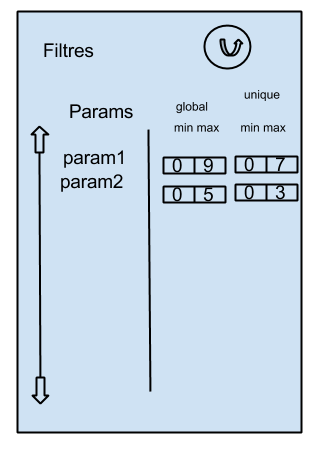
\includegraphics[width=0.35\textwidth]{figure/filtre.png}
			\end{center}
			\caption{Filtre}
			\label{fig:filtre}
		\end{figure}

\subsection{Paramètres de synthèse}

\subsubsection{Les paramètres de base d'ADTool}

ADTool dispose à l'heure actuelle de treize paramètres de base (appelés \textit{domains}), que nous allons présenter succinctement ci-dessous. Nous avons repris les noms (en anglais) qui apparaissent dans le logiciel. 
		
\begin{table*}[!h]
	\centering
	\begin{tabular}{|p{6cm}|p{5cm}|}
  \hline
  \textbf{Paramètre} & \textbf{Valeurs possibles} \\
  \hline
  Difficulty for the proponent (L,M,H) & 
 Low (bas), Medium (moyen), High (élevé) ou l'infini.
\\ \hline
Difficulty for the proponent (L,M,H,E) & 
Low (bas), Medium (moyen), High (élevé), Extreme (extrême) ou l'infini.
\\ \hline
Minimal cost for the proponent (not reusable) & 
Valeurs réelles positives, ou l'infini.\\ \hline
  Minimal skill level needed for the proponent
  & Valeurs entières positives, ou l'infini.\\ \hline
  Minimal time for the proponent (in parallel)
  & Valeurs réelles positives, ou l'infini.\\ \hline
  Minimal time for the proponent (sequential) (\textit{temps minimal séquentiel})
  & Valeurs réelles positives, ou l'infini.\\ \hline
  Overall maximal power consumption & 
  Valeurs réelles positives, ou l'infini.\\ \hline
  Probability of success &
  Valeurs réelles entre 0 et 1.\\ \hline
  Reachability of the proponent's goal in less than k units (in parallel)
  & Valeurs entières de 0 à k. \\ \hline
  Reachability of the proponent's goal in less than k units (sequential)
  & Valeurs entières de 0 à k. \\ \hline
  Satisfiability for the opponent
  & Vrai ou faux. \\ \hline
  Satisfiability for the proponent
  & Vrai ou faux. \\ \hline
  Satisfiability of the scenario
  & Vrai ou faux. \\
  \hline
\end{tabular}
	\caption{Description des paramètres}
	\label{tab:DescriptionParam}
\end{table*}

On voit dans le tableau que des termes particuliers sont utilisés pour désigner les deux parties de l'attaque : l'attaquant et le défenseur. En effet, ADTool permet de se mettre à la place de l'un ou de l'autre. Ainsi, le terme \textit{proponent} désigne l'attaquant (respectivement le défenseur) si on désire son point de vue. L'adversaire (\textit{opponent}) est alors le défenseur (respectivement l'attaquant). % un peu confus. je vois plus un truc du genre : les termes ooponnet et machine designent...

\subsubsection{L'éditeur de paramètres}

L'utilisateur est actuellement cantonné aux valuations présentées ci-dessus et ne peut pas en créer d'autres, ce qui limite ses possibilités d'analyse et d'interprétation. En effet, les paramètres déjà existants ne sont pas les seuls pouvant intéresser un expert en sécurité. Nous souhaitons donc rendre possible la création de nouveaux paramètres, à partir de ceux déjà disponibles et des fonctions mathématiques de base (division, multiplication, min, max, etc). Ces nouvelles valuations pourront ensuite être appliquées à n'importe quel arbre, de la même manière que les paramètres de base. Elles pourront ainsi être utilisées pour analyser les arbres selon de nouveaux critères, et si besoin pour les élaguer à l'aide du filtre que nous allons implémenter.\\

Cette nouvelle fonctionnalité, appelée « Éditeur de paramètres », prendrait donc en entrée les éléments suivants :
\begin{itemize}[label=\ding{170},font=\color{magenta},parsep=0cm,itemsep=0cm]
\item un arbre provenant du projet ;
\item les paramètres intervenant dans la synthèse ;
\item les opérations mathématiques appliquées ;
\item le nom du paramètre de synthèse généré.
\end{itemize}

Par exemple, dans notre arbre illustratif disponible en annexe de ce rapport, nous pouvons voir que les deux sous-arbres « Obtenir illégalement des tickets » (sous-arbre A) et « Falsifier des tickets » (sous-arbre B) permettent d'atteindre l'objectif final. Il est actuellement possible de les valuer par treize paramètres, nous n'en garderons ici que deux pour simplifier : le coût minimal et la probabilité de succès.\\

On constate rapidement que choisir A implique un coût de réalisation moindre pour l'attaquant puisqu'il nécessite peu de matériel. Cependant, un vol est toujours risqué, et les chances de se faire arrêter sont élevées. Opter pour le sous-arbre B, bien que plus cher à réaliser, permet de limiter ces risques : la probabilité de succès est donc plus forte. On voit donc que ces deux paramètres, qui ne sont pas liés, peuvent être tous les deux utiles à l'utilisateur et entraîner une interprétation très différente. C'est pourquoi il serait intéressant de pouvoir les combiner, grâce à notre éditeur de paramètres, afin de les prendre en compte tous les deux. C'est ensuite à l'utilisateur de juger des liens qu'il désire instaurer entre les paramètres : fonctions mathématiques, coefficients, etc.


    \section{Ergonomie du logiciel}
	Des fonctionnalités plus secondaires seront implémentées dans le but de rendre \glasir{} suffisamment ergonomique pour être utilisé avec confort. Ces fonctionnalités n'apporteront pas de nouveautés en terme d'analyse, mais permettront de faciliter la manipulation des arbres dans ADTool et de rendre \glasir{} simple d'utilisation.	

	\subsection{Ouverture simultanée de plusieurs arbres}
		Dans sa version actuelle, ADTool ne permet de travailler que sur un seul arbre à la fois. Cette limitation est assez handicapante : par exemple, l'utilisateur ne peut pas ouvrir deux arbres en même temps pour les comparer. \glasir{} permettra donc d'ouvrir plusieurs instances d'ADTool, chacune contenant un arbre. Ces différentes instances se regrouperont sous la forme d'onglets situés dans l'interface de \glasir{}.
	
	\subsection{Hiérarchie des arbres}
		L'ouverture simultanée de plusieurs arbres induit la possibilité de manipuler un grand nombre d'arbres dans le cadre d'un même projet. Dans le but d'aider l'utilisateur à organiser facilement son projet, \glasir{} fournira dans un dock latéral, une arborescence de dossiers et de sous-dossiers contenant les différents arbres utilisés.

	\subsection{Bibliothèque de modèles}
		Il n'est pas forcément facile pour l'utilisateur de créer un arbre à partir de rien. C'est pourquoi \glasir{} fournira une bibliothèque d'arbres génériques, aidant ainsi l'expert à démarrer son projet. Cette bibliothèque de modèles sera dupliquée pour être propre à chaque nouveau projet, permettant ainsi à l'utilisateur de modifier, compléter ou élaguer les arbres selon ses besoins. Notre étude portant sur le réseau STAR, la bibliothèque de modèles génériques intégrera principalement des ADTrees relatifs aux réseaux de transport en commun rennais. 

		
		Si l'utilisateur construit un nouvel arbre qu'il juge pertinent de réutiliser dans un autre projet, il pourra enregistrer cet arbre comme nouveau modèle, qui se rajoutera donc à la bibliothèque. \glasir{} verra ainsi sa bibliothèque de modèles s'étoffer progressivement au cours du temps.


	
	\subsection{Couper/copier/coller}	
		Actuellement, ADTool ne permet pas l'utilisation des fonctions \emph{couper}/\emph{copier}/\emph{coller}, qui pourraient pourtant s'avérer pratiques lors de la création d'un arbre. Par exemple, dans le cas de l'oubli d'un nœud père, l'instauration de ces fonctionnalités permettrait de déplacer facilement les fils concernés de l'ancien nœud père vers le nouveau.
		
		En conséquence, nous allons modifier ADTool pour qu'il implémente ces fonctionnalités. Ainsi, la sélection d'un nœud entraînera la sélection de ses fils, afin de pouvoir couper ou copier ces nœuds facilement. Les raccourcis clavier \og classiques \fg{}  de ces fonctions (\emph{CTRL+X, CTRL+C, CTRL+V}) seront mis en place.


	\subsection{Amélioration du codage des arbres}
		ADTool affiche actuellement dans son interface une section nommée \emph{ADTerm Edit}. Celle-ci contient une représentation de l'arbre sous un format texte, en utilisant un langage propre au logiciel. Lors de la modification de l'arbre dans l'éditeur graphique, ADTool met à jour le texte correspondant en temps réel et de manière automatique. L'inverse est également vrai : il est possible de changer les labels des nœuds, ou les opérateurs, directement depuis \emph{ADTerm Edit} afin d'afficher ensuite le résultat graphiquement.

		Mais le langage qui permet de décrire les arbres sous format texte n'est pas très lisible : il ne contient par exemple pas le nom des nœuds autres que les feuilles. Sur la {\sc Figure} \ref{fig:int_adTool}, on peut constater que le code indique le nom des deux feuilles \og Acheter le matériel nécessaire \fg{} et \og Essayer les clés possibles \fg{}, et que la conjonction est bien précisée par l'opérateur \og ap \fg{} (\og op \fg{} en cas de disjonction). Mais aucune référence n'est faite au label du nœud père \og Casser le chiffrage \fg{}. Nous modifierons la grammaire pour corriger ce défaut, afin de rendre l'utilisation de cette fenêtre plus intuitive.

		\begin{figure}[h]
			\centering
			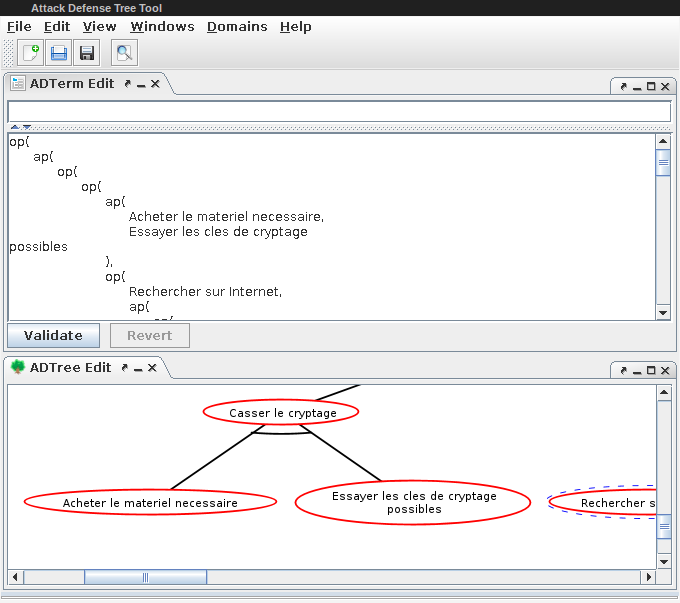
\includegraphics[width=0.6\textwidth]{figure/interface_adtool.png}
			\caption{L'interface d'ADTool. En haut, l'arbre au format texte ; en bas, sa représentation graphique.}
			\label{fig:int_adTool}
		\end{figure}
	
	\subsection{Annulation d'une action}	
		Pour le moment, effectuer une action sous ADTool est irréversible. Cela n'est pas grave pour certaines actions rapides à effectuer, telles que le renommage d'un nœud. Mais supprimer un nœud (ce qui implique la disparition de tous ses nœuds fils s'il y en a) par erreur peut entraîner un travail énorme, et donc une perte de temps. La possibilité de revenir à l'état précédent de l'arbre (par le raccourci clavier classique \emph{CTRL+Z}) éviterait d'avoir à refaire ce travail de construction fastidieux. Nous souhaitons créer au moins une sauvegarde de l'état précédent, afin de pouvoir annuler la dernière modification effectuée. Si possible, nous envisageons l'implémentation d'une pile circulaire contenant les N derniers états (chaque modification entraînant la création d'un nouvel état) avec un curseur pointant sur l'état courant. Cela permettrait de revenir en arrière sans contraintes. 

		Cette fonctionnalité sera implémentée en utilisant le patron de conception \emph{Commande}. Les actions de l'utilisateur dans ADTool seront sauvegardées pour pouvoir, quand l'utilisateur demandera l'annulation de son action, effectuer l'action inverse. 

	\subsection{Vue globale des paramètres}
		Dans l'état actuel d'ADTool, lorsqu'un arbre est valué, un seul paramètre est affiché (le même pour tous les nœuds) même si plusieurs paramètres sont utilisés en réalité. En effet, chaque valuation a un onglet propre, dans lequel elle est la seule effectivement affichée sur l'arbre. Nous souhaitons créer un onglet plus général, dans lequel tous les paramètres voulus peuvent être visibles sur l'arbre en simultané. C'est ensuite à l'expert de décider des paramètres qu'il juge utile d'afficher. Cela serait aussi valable pour les paramètres de synthèse évoqués dans la {\sc Sous-section} \ref{subsection:synthese}.
	
		Pour une meilleure lisibilité, chaque paramètre aura une couleur différente, et l'arbre sera accompagné d'une légende résumant ce jeu de coloration et ses correspondances. Nous devrons également gérer la taille des nœuds, pour que les paramètres ne dépassent pas de la bulle. Un tel système étant déjà présent dans ADTool pour gérer les labels, il suffira de l'étendre à l'affichage des paramètres.

		Maintenant que les différentes fonctionnalités à développé ont été défini, une première planification peut être présentée. 

    \section{Organisation}
	\label{sec:orga}
	\subsection{La méthode SCRUM}
		\label{subsec:scrum}

	Afin de définir la méthode de gestion de projet à mettre en place pour la réalisation de \glasir{}, nous avons débattu ensemble des différentes méthodes à notre disposition. A la suite de 	nos discussions en réunions, nous nous sommes dirigés vers une méthode agile proche du \og \textsc{scrum} \fg{}. Ce choix s'est fait sur les points qui sont détaillé ci-dessous :

	L'organisation des rôles que nous avons mise en place depuis le début du projet se base sur un rôle de \og Coordinateur \fg{}, qui est responsable de la réalisation et du rendu d'un livrable (rapport, version logicielle, etc). Ce rôle tourne à chaque nouveau livrable, de sorte que chacun des membres de l'équipe l'exerce au moins une fois. Le rôle de coordinateur que nous avons défini nous a donc semblé correspondre au rôle de ScrumMaster tel que défini dans la méthode \textsc{scrum}.

	Le coordinateur endosse également la responsabilité de Product Owner, qu'il partage avec les encadrants du Projet pour ce qui est de la définition des Objectifs et surtout de l'acceptation des livrables.

	En place de la mêlée quotidienne du \textsc{scrum}, nous nous réunissons une fois par semaine afin de discuter de l'avancement de nos tâches respectives et faire part de nos difficultés. Nous avons décidé d'adopter un rythme hebdomadaire plutôt que quotidien car nous ne travaillerons pas à temps plein sur le projet et ce rythme nous a donc semblé plus adéquat. Nous définissons en fonction des retours en réunion les éventuels ajustements à effectuer la semaine suivante et dans le reste de la planification.

	Enfin, chaque version sera composée de sprints au cours desquels nous nous consacrerons à un sous-ensemble de tâches nécessaires à la réalisation d'une version de \glasir{}. Ces tâches constitueront les Users Stories du projet, et sont détaillées dans la \textsc{sous-section}~\ref{subsec:taches_unitaires}.  
	
	\subsection{Tâches unitaires et estimations}
		\label{subsec:taches_unitaires}

	Nous avons décidé de livrer trois versions de \glasir{} : deux intermédiaires et une finale. Ces dernières ont elles-mêmes été divisées en tâches unitaires, décrites dans cette section.
	
	Pour déterminer le temps nécessaire à l'accomplissement de chaque tâche, nous avons combiné les méthodes d’estimation \og Analogique \fg{} et \og Expertise \fg{}. En effet, la méthode \og Analogique \fg{} consiste à estimer la durée d'une tâche par analogie avec une tâche similaire déjà effectuée (au sein d'un autre projet par exemple). La méthode \og Expertise \fg{}, quant à elle, repose sur le jugement d'un expert. Bien qu'aucun membre de notre groupe ne puisse réellement se considérer comme tel, nos stages respectifs ont tout de même permis d'apporter des avis constructifs sur l'estimation de la durée des tâches.
	
	Les résultats de ces différentes estimations sont décrits ci-après pour chaque version. Il est à noter que les tests et la rédaction de la documentation sont pris en compte dans l'estimation du temps nécessaire à la réalisation de chacune des tâches.
	

		\subsubsection{Version 0.1}
			Huit grandes tâches ont été identifiées pour cette version et sont présentées dans la {\sc Table} \ref{tab:taches_units_1}. 
			\begin{table}[H]
				\centering
				\begin{tabular}{|c|r|l|c|r|}
					\hline
					\textbf{Cible} & \textbf{Id} & \textbf{Tâche} & \textbf{Technologies} & \textbf{Durée}\\
					\hline

					\multirow{5}{*}{\glasir{}} & 1.1 & Squelette interface & WPF & 6h\\
					\cline{2-5}
					 & 1.2 & Gestion fichiers projet & C++ & 20h\\
					\cline{2-5}
					 & 1.3 & Intégration ADTool dans \glasir & JNI & 20h\\
					\cline{2-5}
					 & 1.4 & \'Evaluateur de fonction & Java & 12h\\
					\cline{2-5}
					 & 1.5 & Interface évaluateur & WPF & 8h\\
					\hline

					\multirow{3}{*}{ADTool} & 1.6 & Valuation ADTrees & \multirow{3}{*}{Java} & 18h\\
					\cline{2-3} \cline{5-5}
					 & 1.7 & Refonte langage des ADTrees & & 16h\\
					\cline{2-3} \cline{5-5}
					 & 1.8 & Vue globale des paramètres & & 12h\\
					\hline

					\multicolumn{4}{|l|}{\bf Total} & {\bf 112h}\\
					\hline
				\end{tabular}
				\caption{Tâches associées à la version 0.1.}
				\label{tab:taches_units_1}
			\end{table}
			
			
			La réalisation de cette version sera découpée en trois sprints, présentés ci-dessous :

			\noindent\textbf{Sprint 1} Création de l'interface utilisateur de base de \glasir{}, intégration du logiciel ADTool en tant que fenêtre de \glasir{}, possibilité de création d'un nouveau projet et sa sauvegarde, affichage des différents arbres d'un projet dans un dock sous forme d'arborescence.\newline
			\textbf{Sprint 2} Reconnaissance d'une formule mathématique par le logiciel ADTool, création d'un paramètre en fonction de l'évaluation de cette formule, et l'amélioration de la représentation des arbres sous forme d'une grammaire au sein d'ADTool.\newline
			\textbf{Sprint 3} Affichage de plusieurs paramètres par nœud d'un arbre, possibilité de communication entre le module éditeur de fonction de \glasir{} et la partie création d'un paramètre de synthèse implémentée précédemment dans ADTool.\newline


		\subsubsection{Version 0.2}
			Le développement de la version 0.2 est découpé en cinq tâches, visibles dans la {\sc table} \ref{tab:taches_units_2}.
			\begin{table}[h]
				\centering
				\begin{tabular}{|c|r|l|c|r|}
					\hline
					\textbf{Cible} & \textbf{Id} & \textbf{Tâche} & \textbf{Technologies} & \textbf{Durée}\\
					\hline

					\multirow{4}{*}{\glasir{}} & 2.1 & Algorithme filtrage & C++ & 24h\\
					\cline{2-5}
					 & 2.2 & Interface filtre & WPF & 15h\\
					\cline{2-5}
					 & 2.3 & Multiples instances d'ADTool & C++, WPF & 20h\\
					\cline{2-5}
					 & 2.4 & Affichage arbre filtré & Java, WPF & 16h\\
					\hline

					\multirow{1}{*}{ADTool} & 2.5 & Couper/copier/coller & \multirow{1}{*}{Java} & 25h\\
					\hline

					\multicolumn{4}{|l|}{\bf Total} & {\bf 100h}\\
					\hline
				\end{tabular}
				\caption{Tâches associées à la version 0.2.}
				\label{tab:taches_units_2}
			\end{table}
			
			Nous avons réparti les tâches en trois sprints :

			\noindent\textbf{Sprint 4} Implémentation de l'algorithme de filtrage, permettre l'ouverture de plusieurs instances d'ADTool au sein de différents onglets de l'interface de \glasir{}.\newline 
			\textbf{Sprint 5} Affichage du panneau relatif à ce module au sein de l'interface utilisateur de \glasir{}. Implémentation de la fonction couper/copier-coller.\newline % ou durant le snd sprint?
			\textbf{Sprint 6} Affichage de l'arbre filtré.

		\subsubsection{Version 1.0}
			Quatre tâches ont été identifiées pour la version 1.0 de \glasir{}, regroupées dans la {\sc Table} \ref{tab:taches_units_3}.
			\begin{table}[h]
				\centering
				\begin{tabular}{|c|r|l|c|r|}
					\hline
					\textbf{Cible} & \textbf{Id} & \textbf{Tâche} & \textbf{Technologies} & \textbf{Durée}\\
					\hline

					\multirow{4}{*}{\glasir{}} & 3.1 & Optimiseur & C++, WPF & 30h\\
					\cline{2-5}
					 & 3.2 & Bibliothèque de modèles & C++, WPF & 20h\\
					\cline{2-5}
					 & 3.3 & Harmonisation interface & WPF & 16h\\
					\cline{2-5}
					 & 3.4 & Packaging & ? & 8h\\
					\hline

					\multirow{1}{*}{ADTool} & 3.5 & Ctrl-Z & \multirow{1}{*}{Java} & 16h\\
					\hline

					\multicolumn{4}{|l|}{\bf Total} & {\bf 90h}\\
					\hline
				\end{tabular}
				\caption{Tâches associées à la version 1.0.}
				\label{tab:taches_units_3}
			\end{table}
			
			Les sprints se composeront de :

			\noindent\textbf{Sprint 7} Implémentation de l'algorithme de l'optimiseur, création d'une bibliothèque de modèles.\newline
			\textbf{Sprint 8} Affichage du panneau de l'optimiseur dans \glasir{}, possibilité d'annuler une action dans ADTool.\newline
			\textbf{Sprint 9} Harmonisation de l'interface et réalisation du packaging. \newline

		%TODO estimations
	\subsection{Organisation du groupe et répartition des tâches}
		Lors de la phase de développement de \glasir{}, notre groupe de projet sera réduit à trois étudiants : Pierre-Marie {\sc Airiau}, Valentin {\sc Esmieu} et Maud {\sc Leray}. Les trois autres, Florent {\sc Mallard}, Hoel {\sc Kervadec} ainsi que Corentin {\sc Nicole}, partiront en effet étudier à l'étranger.
		
		Nous comptons donc nous répartir les tâches selon trois composantes générales : Maud L. travaillera principalement sur ADTool, Pierre-Marie A. sur les algorithmes et sur l'interfaçage entre ADTool et \glasir{}, et Valentin E. s'orientera sur l'interface utilisateur de \glasir{}. La {\sc Table} \ref{table:repartition} donne la répartition des tâches plus en détails.
			


		\begin{table}[H]
			\centering
			\begin{tabular}{|l|c|r||c|r||c|r|}
				\hline
				\multirow{2}{*}{} & \nomRepart{Pierre-Marie A.} & \nomRepart{Valentin E.} & \nomRepartt{Maud L.}\\
				\cline{2-7}
				 & {\bf Id tâche} & {\bf Durée} & {\bf Id tâche} & {\bf Durée} & {\bf Id tâche} & {\bf Durée}\\
				\hline
				{\bf Version 0.1} & - & {\bf 38h} & - & {\bf 34h} & - & {\bf 40h}\\
				 & 1.3 & 10h & 1.1 & 6h & 1.2 & 10h\\
				 & 1.4 & 12h & 1.2 & 10h & 1.6 & 18h\\
				 & 1.7 & 16h & 1.3 & 10h & 1.8 & 12h\\
				 & - & - & 1.5 & 8h & - & -\\
				\hline
				{\bf Version 0.2} & - & {\bf 39h} & - & {\bf 33h} & - & {\bf 28h}\\
				 & 2.1 & 24h & 2.3 & 20h & 2.4 & 16h\\
				 & 2.2 & 15h & 2.5 & 13h & 2.5 & 12h\\
				\hline
				{\bf Version 1.0} & - & {\bf 25h} & - & {\bf 23h} & - & {\bf 42h}\\
				 & 3.1 & 15h & 3.1 & 15h & 3.2 & 10h\\
				 & 3.2 & 10h & 3.4 & 8h & 3.3 & 16h\\
				 & - & - & - & - & 3.5 & 16h\\
				\hline
				{\bf Total} & \multicolumn{2}{r||}{{\bf 102h}} & \multicolumn{2}{r||}{{\bf 100h}} & \multicolumn{2}{r|}{{\bf 110h}}\\
				\hline
			\end{tabular}
			\caption{Répartition des tâches, par personne et par version.}
			\label{table:repartition}
			\label{tab:repartition}
		\end{table}


	\subsection{Risques}
		\label{subsec:risques}

	%L'implémentation d'un logiciel comporte toujours des risques. Afin de ne pas nous laisser surprendre par ces derniers, nous avons cherché à lister ceux qui nous venaient à l'esprit.

    % Pour que notre projet se déroule le mieux possible, nous avons listé certains événements susceptibles de nous faire prendre du retard. Ils sont répertoriés dans le tableau\ref{fig:risques}, avec les tâches qu'ils concernent. Nous leur avons ajouté les notions de probabilité (Pr) et de criticité (Cr), sur une échelle de 1 à 3 : 1 pour faible, 2 pour moyenne, 3 pour élevée. Enfin, la dernière colonne cite des solutions possibles pour contre les risques énoncés.

    Dans le but de délivrer ce projet dans les délais, une évaluation des risques a été effectuée. Celle-ci a pour but d'identifier les différents facteurs qui pourraient engendrer des difficultés dans la réalisation des tâches et entraîner ainsi un retard, ou une incapacité à implémenter une partie du cahier des charges. Nous avons associé à chaque élément de cette liste les notions de probabilité (Pr) et de criticité (Cr), sur une échelle de 1 à 3 : 1 pour faible, 2 pour moyenne, 3 pour élevée. Dans le but de réagir au mieux en cas d’apparition de ces aléas, des solutions ont été définies. Le résultat de cette réflexion est présenté dans la \textsc{table}~\ref{fig:risques}. 


	\begin{table}[H]
		\centering
		\begin{tabular}{|p{4cm}|l|l|l|p{4cm}|}
		\hline
            \textbf{Risque} & \textbf{Tâches concernées} & \textbf{Pr.} & \textbf{Cr.} & \textbf{Solution}\\
            \hline
            Mauvaise estimation des durées nécessaires aux tâches unitaires & 
                Toutes & 3 & 3 &
                Bien s'organiser et respecter les délais\\ 
            \hline
            Apparition d'un bug difficile à corriger & 
                Toutes & 3 & 3 &
                Faire des tests unitaires\\
            \hline
            Difficulté à créer une grammaire & 
                1.4 & 1 & 2 &
                Simplifier les expressions à évaluer\\ 
            \hline
            Manque de connaissances techniques & 
                Toutes & 3 & 3 &
                Approfondir nos connaissances\\ 
            \hline
            Rédaction trop tardive de la documentation & 
                Toutes & 2 & 1 &
                Commenter le code au fur et à mesure\\
            \hline
            Mauvaise compréhension du code d'ADTool & 
                Toutes celles sur ADTool & 2 & 2 &
                Contacter le développeur d'ADTool\\ 
            \hline
            Mauvaise communication entre ADTool et \glasir{} & 
                1.4, 2.1, 3.1 & 2 & 3 &
                Utiliser le fichier XML lisible par ADTool\\ 
            \hline
            Perte de temps sur une tâche secondaire & 
                Toutes & 2 & 1 &
                Compter ses heures, faire le point lors des réunions\\ 
            \hline
            Algorithme ralentissant le logiciel & 
                3.1, 2.2 & 1 & 1 &
                Optimiser l’algorithme\\ 
            \hline
            Échec de l'intégration d'ADTool dans \glasir{} & 
                1.2 & 1 & 3 &
                Lancer ADTool séparément\\ 
            \hline
		\end{tabular}
		\caption{Tableau des risques}
		\label{fig:risques}
	\end{table}
	

    \section{Critiques}
	Après la rédaction du rapport précédent (pré-étude), nous avions constaté que notre organisation de travail était à revoir. 
	En effet, nous avions trop cloisonné la rédaction des différentes parties, et il nous manquait un superviseur chargé d'harmoniser le tout.
	Le résultat fut un rapport dont les parties ne s'enchaînaient pas toujours correctement, et avec des styles de rédaction très variables : cela manquait d'homogénéité.

	De plus, nous avions trop tardé à faire nos \og brainstorming \fg~ pour déterminer précisément ce que nous allions faire, ce qui a grandement retardé la rédaction. Nous avons même dû supprimer une partie de notre travail.

	À partir de ces constats, nous avons décidé de démarrer ce deuxième rapport par une série de réunions. Cela nous a permis de commencer la rédaction en ayant une idée précise de ce que nous allions écrire.
	Cette fois, nous avons désigné un responsable d'harmonisation, Corentin Nicole, qui rédige moins mais s'assure de la cohérence globale du rapport tout au long de son avancement.

% ABSENCE DE REFERENCES

    % On a pas de conclusion :o

    \includepdf[angle=90]{figure/pre_optimiseur.pdf}

    % a eviter
    \nocite{*}

    \bibliographystyle{plain}
    \bibliography{input/biblio}

    % Manoucherie incoming
    \pagevierge
    \ifthenelse{\isodd{\thepage}}
    {\pagevierge}
    {}
    
\includepdf[pages=2]{figure/couv.pdf}

\end{document}
